\subsection{Decision Trees}

The idea of a decision tree is to split the classifications into a set of decisions.
The first 50 PCA values are used and by looking at the deviance for each split a tree can be created.

\begin{figure}[h]
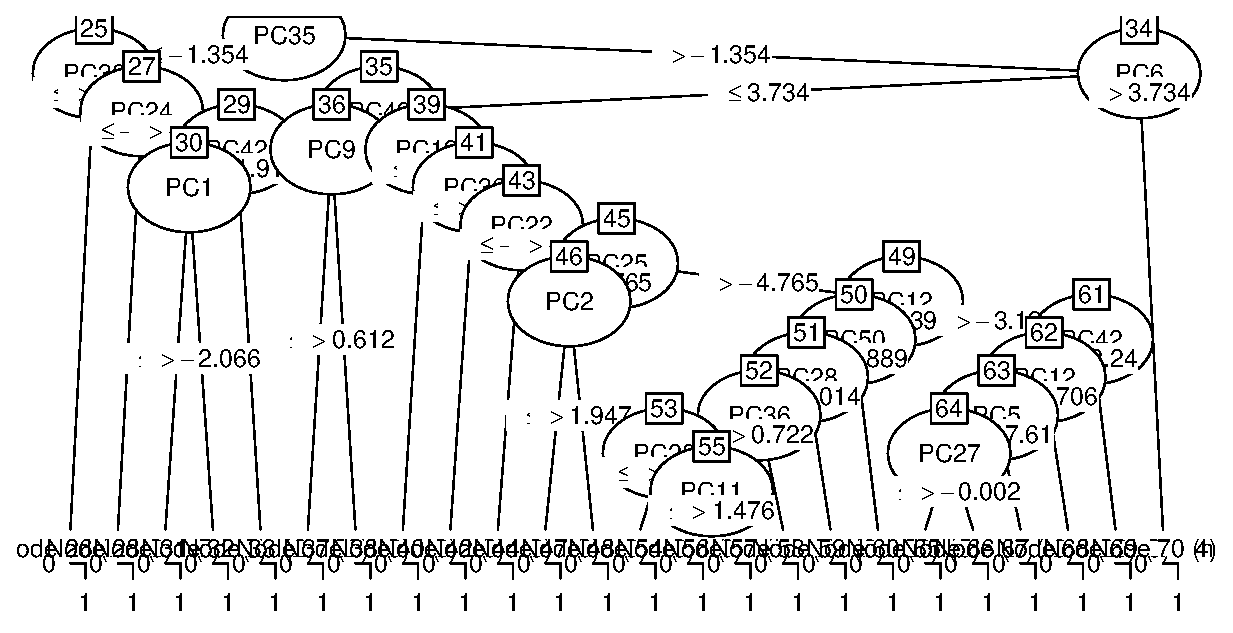
\includegraphics[width = \textwidth]{graphics/tree_section}
\caption{Small section of the tree}
\label{fig:tree_section}
\end{figure}

Building a tree can be done using the ``C50'' library in R.
The tree with the training data of 15 people (56000 cases) contains 6338 nodes.
A small section of the tree is shown in figure \ref{fig:tree_section}.
Each node shows which principal component and the split to which the decision is made.
Each leaf shows the probability of a classification.\\
The classifications is shown in table \ref{tb:tree_confus}.

\begin{table}[H]
    \centering
    \begin{subtable}{0.005\textwidth}
    \end{subtable}
    \begin{subtable}{0.8\textwidth}
        \centering
        
\begin{tikzpicture}
            \node at (0,0) {};
            \node at (1,0) {\Large Actual Class}; 
        \end{tikzpicture}
    \end{subtable}

    \begin{subtable}{0.005\textwidth}
        \flushright
        
\begin{tikzpicture}
            \node[rotate=90] {\Large Predicted Class};
        \end{tikzpicture}
    \end{subtable}
    \begin{subtable}{0.8\textwidth}
        \begin{subtable}{\textwidth}
            \centering
            \begin{tabular}{*{11}{c}}
                &0	& 1	& 2	& 3	& 4	& 5	& 6	& 7	& 8	& 9 \\
\hline
0	& 348	& 1	& 0	& 0	& 3	& 4	& 7	& 2	& 2	& 2 \\
1	& 0	& 349	& 3	& 2	& 4	& 0	& 1	& 1	& 1	& 3 \\
2	& 2	& 2	& 347	& 3	& 3	& 2	& 1	& 2	& 2	& 1 \\
3	& 0	& 1	& 3	& 346	& 1	& 1	& 0	& 2	& 5	& 1 \\
4	& 2	& 0	& 1	& 0	& 338	& 8	& 0	& 2	& 1	& 0 \\
5	& 1	& 0	& 0	& 3	& 5	& 342	& 1	& 2	& 1	& 2 \\
6	& 3	& 6	& 0	& 0	& 1	& 1	& 348	& 2	& 3	& 3 \\
7	& 1	& 0	& 1	& 3	& 1	& 1	& 0	& 342	& 2	& 5 \\
8	& 2	& 0	& 3	& 2	& 0	& 1	& 1	& 3	& 338	& 5 \\
9	& 1	& 1	& 2	& 1	& 4	& 0	& 1	& 2	& 5	& 338 \\

            \end{tabular}
            \caption{Confusion table of decision tree}
            \label{tb:tree_confus}
        \end{subtable}
    \end{subtable}
\end{table}

\begin{figure}[h]
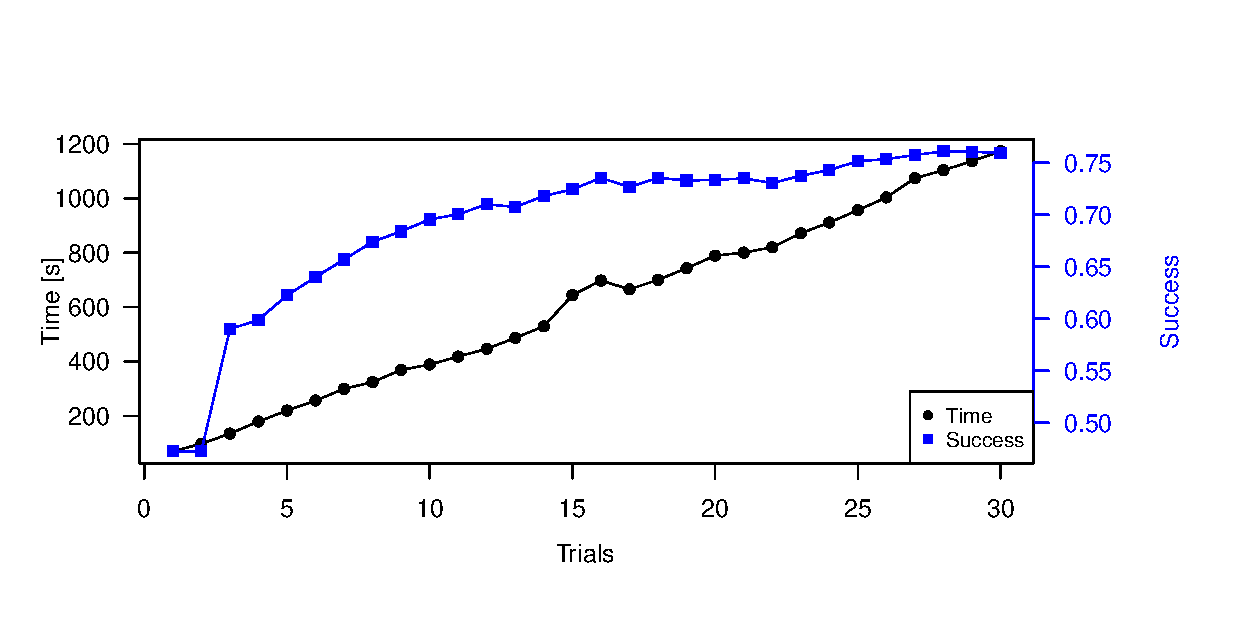
\includegraphics[width = \textwidth]{graphics/tree_timing}
\caption{Performance of boosting the C50 algorithm. The test person is G3M2 and training data everyone else.}
\label{fig:tree_timing}
\end{figure}

The ``C50'' function provides a boosting function.
Boosting is a process in which the algorithm is training with the train data with multiple trials to increase performance.
This is expected to take more time but improve performance.
In figure \ref{fig:tree_timing} can the success be seen of multiple trials.
Since the algorithm trains towards a good performance on the train data it can be over-fitted as seen when the number of trails exceed 20. 
The timing is as expected linear dependent on the number of trials.

To test the overall performance each person was used as test data to see how they successful the data could be classified.
The training set consist of all people with the person in the test set is removed from the training set. 
The data is normalized before PCA and the first 50 PC is used. 
In figure \ref{fig:tree_success_all} is the success of all people shown.
The trees are boosted with 15 trials.

\begin{figure}[h]
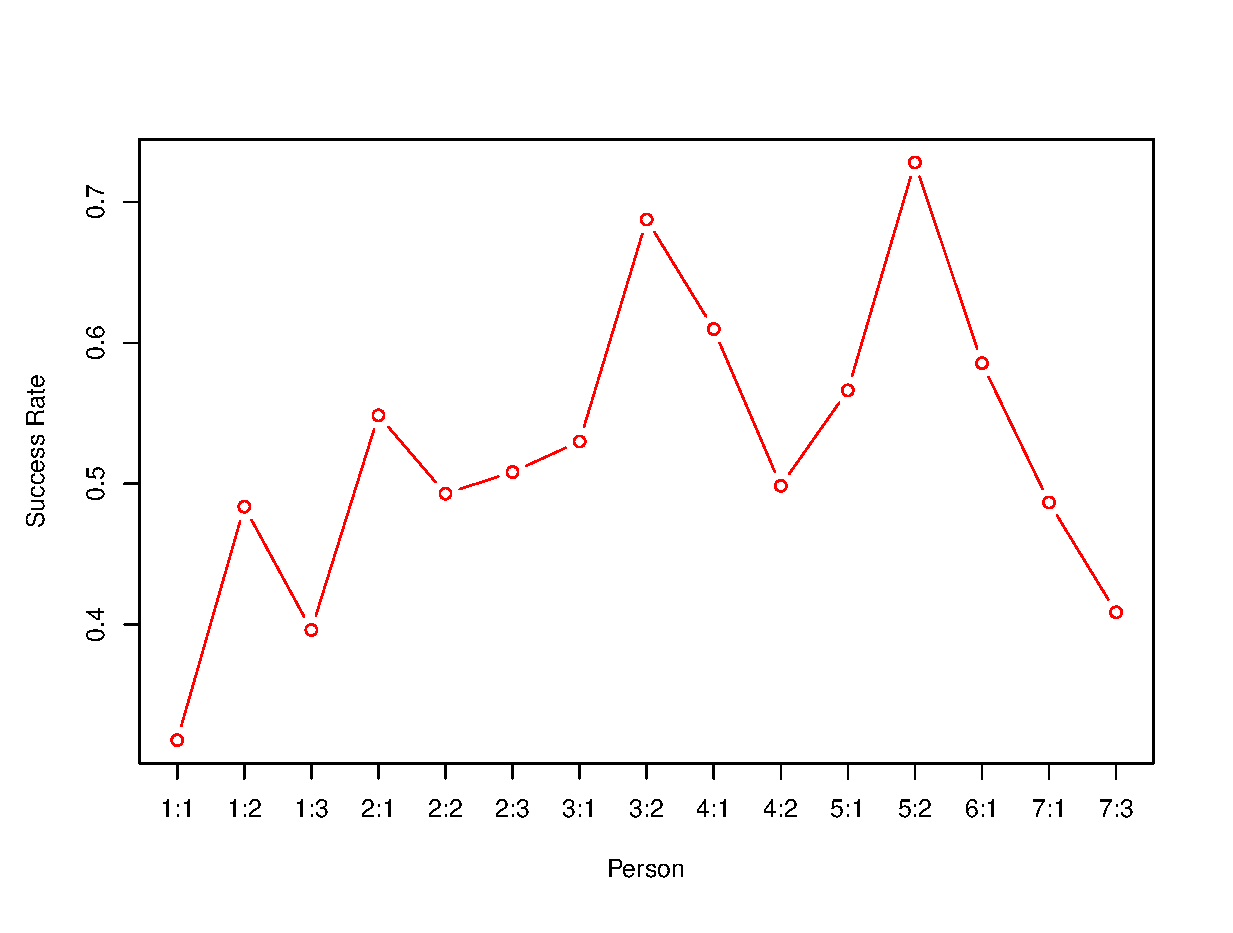
\includegraphics[width = \textwidth]{graphics/tree_success_all}
\caption{Success of decision tree on all people.}
\label{fig:tree_success_all}
\end{figure}
